\documentclass{cours}

\usepackage{tikz}
\usetikzlibrary{arrows.meta}

\title{Continuité des Fonctions d'une \\ Variable Réelle}
\author{Diego Van Overberghe}

\begin{document}
    \maketitle{2}

    \begin{Gpartie}{Définition}
        Soit $f$, définie sur un intervalle $I$, et soit $a$, un réel de $I$.
        La fonction $f$ est continue si et seulement si : \[\lim_{x \to a} f(x)=f(a)\]
        $f$ est continue sur l'intervalle $I$, si et seulement si, quel que soit le réel $x\in I$, $f$ est continue en $x$.

        H.P.: $\forall\epsilon >0,\ \exists\alpha >0,\ \forall x\in\big]a-\alpha\,; a+\alpha\big[,\, f(x)\in\big]f(a)-\epsilon\,; f(a)+\epsilon\big[$
        \begin{Spartie}{Exemple}
            La fonction inverse est continue sur $\big]-\infty\,;0\big[$, et sur $\big]0\,;+\infty\big[$.\\
            La fonction ``Partie Entière'' est définie sur $\mathbb{R}$, mais pas continue sur $\mathbb{R}$. \\[2ex]
            \begin{center}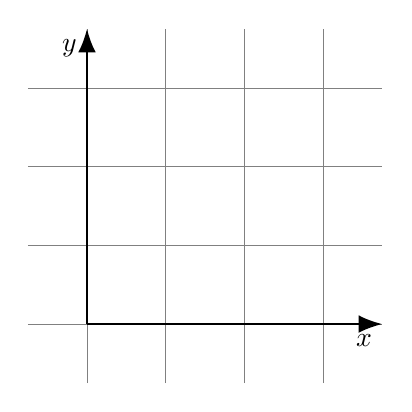
\begin{tikzpicture}
                \draw[gray,very thin] (-.75,-.75) grid (3.75,3.75);
                \draw[thick, -{Latex[length=3mm]}] (0,0) -- (3.75,0) node[anchor=north east] {$x$};
                \draw[thick, -{Latex[length=3mm]}] (0,0) -- (0,3.75) node[anchor=north east] {$y$};
            \end{tikzpicture}\end{center}
            \parbox{\linewidth}{\captionof{figure}{\centering Représentation Graphique de la Fonction \linebreak ``Partie Entière'', continue sur $\big[n\,;n+1\big[$ avec $n\in\mathbb{Z}$.}}
            \begin{center}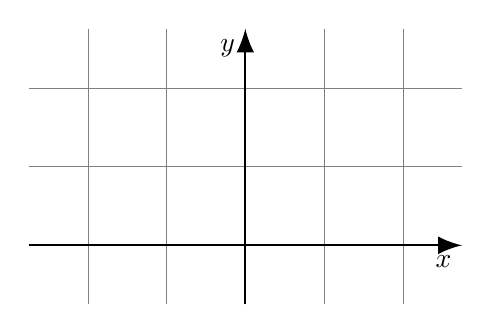
\begin{tikzpicture}
                \draw[gray, very thin] (-2.75,-.75) grid (2.75,2.75);
                \draw[thick, -{Latex[length=3mm]}] (-2.75,0) -- (2.75,0) node[anchor=north east] {$x$};
                \draw[thick, -{Latex[length=3mm]}] (0,-.75) -- (0,2.75) node[anchor=north east] {$y$};
            \end{tikzpicture}\end{center}
            \parbox{\linewidth}{\captionof{figure}{Représentation Graphique de la Fonction Absolue}}
        \end{Spartie}

        \begin{Spartie}{Propriété}
            La somme, le produit et la composée de deux fonctions continues est continue. \\
            L'inverse d'une fonction continue est continue sur tout intervalle où elle ne s'annule pas.
            \[f : x\mapsto x^2\quad\text{continue}\] \[g : x\mapsto\dfrac{1}{x^2}\quad\text{Définie sur }\mathbb{R}^*\text{, continue sur }\big]-\infty\,;0\big[\text{ et }\big]0\,;+\infty\big]\]
        \end{Spartie}
    \end{Gpartie}

    \hspace{4ex}

    \begin{Gpartie}{Théorème des Valeurs Intermédiaires}
        \begin{Spartie}{Théorème}
            Si une fonction $f$ est continue sur un intervalle $\big[a\,;b\big]$ alors, pour tout réel $k\in\Big[\text{min}\big(f(a)\,;f(b)\big)\,;\text{max}\big(f(a)\,;f(b)\big)\Big]$ il existe au moins un réel $c\in\big[a\,;b\big]$ tel que $f(c)=k$ \\
            C'est-à-dire, pour tout réel $k$, compris entre $f(a)$ et $f(b)$, il existe un réel $c\in\big[a\,;b\big]$ tel que $f(c)=k$
            \begin{center}
                %\begin{tikzpicture}
                    \noindent\includegraphics[width=6cm]{example-image}
                    \parbox{\linewidth}{\captionof{figure}{Exemple du Théorème des Valeurs Intermédiaires}}
                %\end{tikzpicture}
            \end{center}
            Pour tout $k$ appartenant à $\big[f(b)\,;f(a)\big]$, il existe au moins un réel $c\in\big[a\,;b\big]$, tel que $f(c)=k$
        \end{Spartie}
        \begin{Spartie}{Corollaire}
            Si une fonction $f$ est continue et strictement monotone sur un intervalle $\big[a\,;b\big]$, alors, pour tout $k\in\Big[\text{min}\big(f(a)\,;f(b)\big)\,;\text{max}\big(f(a)\,;f(b)\big)\Big]$, il existe un \textit{unique} réel $c\in\big[a\,;b\big]$, tel que $f(c)=k$. 
            \begin{center}
                % \begin{tikzpicture}
                    \noindent\includegraphics[width=6cm]{example-image}
                    \parbox{\linewidth}{\captionof{figure}{\centering Illustration du Corollaire du Théorème \linebreak des Valeurs Intermédiaires}}
                % \end{tikzpicture}
            \end{center}
            \begin{SSpartie}{Cas Particulier}
                Si une fonction $f$ est continue sur un intervalle $\big[a\,;b\big]$, et si $f(a)$ et $f(b)$ sont de signes contraires, alors il existe au moins une solution à $f(x)=0$, sur $\big[a\,;b\big]$.
            \end{SSpartie}
        \end{Spartie}
    \end{Gpartie}
\end{document}